\documentclass[12pt]{article}

\usepackage{booktabs}
\usepackage{dcolumn} 
\usepackage{epstopdf}
\usepackage{graphicx}
\usepackage{hyperref}
\usepackage{longtable} 
\usepackage{natbib}
\usepackage{rotating}
\usepackage{tabularx}
\usepackage{amsmath}
\usepackage{setspace}
\usepackage{caption}
\usepackage{epigraph}

\usepackage[super]{nth}  
\hypersetup{
  colorlinks = TRUE,
  citecolor=blue,
  linkcolor=red,
  urlcolor=black
}

\hypersetup{colorlinks = TRUE, citecolor=blue, linkcolor=red, urlcolor=black}

\DeclareMathOperator*{\argmax}{arg\,max}

\newcommand{\starlanguage}{Significance indicators: $p \le 0.05:*$, $p \le 0.01:**$ and $p \le .001:***$.}

\newcommand{\covid}{COVID-19}  

\newtheorem{proposition}{Proposition}
\newtheorem{assumption}{Assumption}
\newtheorem{example}{Example}
\newtheorem{observation}{Observation}
\newtheorem{lemma}{Lemma}

\newcommand{\important}[1]{\textcolor{blue}{\textbf{ #1}}}
\newcommand{\quantclaim}[1]{\textcolor{red}{\textbf{ #1}}}


\newcommand{\LFPRhat}{58}
\newcommand{\numObs}{4,946}
\newcommand{\numObsWorking}{2,845}
\newcommand{\SurveyStart}{2020-06-29}
\newcommand{\SurveyEnd}{2020-07-04}
\newcommand{\LaidOff}{8.0}
\newcommand{\LaidOffLB}{4.5}
\newcommand{\LaidOffUB}{11.5}
\newcommand{\WFH}{28.4}
\newcommand{\WFHLB}{25.3}
\newcommand{\WFHUB}{31.5}
\newcommand{\alreadyWFH}{14.3}
\newcommand{\alreadyWFHLB}{10.9}
\newcommand{\alreadyWFHUB}{17.7}
\newcommand{\stillCommute}{42.7}
\newcommand{\stillCommuteLB}{40.0}
\newcommand{\stillCommuteUB}{45.5}


\begin{document} 



\title{COVID-19 and Remote Work:\\ An Early Look at US Data\footnote{
    MIT's COUHES ruled this project exempt (project number E-2075).
    {Code \& Data: \href{https://github.com/johnjosephhorton/remote\_work/}{https://github.com/johnjosephhorton/remote\_work/}}.
    Thanks to Sam Lord for helpful comments. 
  }}

\date{\today}

\date{\today}

\author{Erik Brynjolfsson\\MIT, Stanford \& NBER \and John Horton\\MIT \& NBER \and Adam Ozimek\\Upwork \and Daniel Rock\\MIT \and Garima Sharma\\MIT \and Hong Yi Tu Ye\\MIT}


\maketitle

\begin{abstract}
  \noindent 
  We report the results of a nationally representative sample of the US population on how they are adapting to the \covid{} pandemic.
  The survey ran from April 1-4, 2020.
  Of those previously employed, \WFH{}\% report they were commuting and are now working from home.
  In addition, \LaidOff{}\% report being laid-off or furloughed in the last 4 weeks.   
  %The percentage already working from home pre-\covid{} is \alreadyWFH{}\% (95\% CI is [\alreadyWFHLB,\alreadyWFHUB]). 
  There is a strong negative relationship between the fraction in a state still commuting to work and the fraction working from home which suggests that many workers currently commuting could be converted to remote workers.
  Furthermore, using data on state unemployment insurance (UI) claims, we find that states with higher fractions of remote workers have higher-than-expected UI claims.
  \newline 
\end{abstract} 

\onehalfspacing 

\section{Introduction}
The on-going \covid{} pandemic has confined large numbers of people to their homes via quarantines and shelter-in-place orders.
Large numbers of businesses are closed. 
There have already been enormous and unprecedented increases in workers filing unemployment insurance claims \citep{goldsmith2020}. 
To get a real-time sense of how firms and workers are responding, we conducted a survey using Google Consumer Surveys (GCS).\footnote{
GCS is a relatively low-cost tool for rapidly collecting responses to simple questions \cite{stephens2014hands}, and response representativeness is often comparable to similar alternatives \citep{santoso2016survey, brynjolfsson2019using}.
}

We asked a single question:
````Have you started to work from home in the last 4 weeks?''
with the following response options: 
\begin{enumerate} 
\item ``I continue to commute to work''
\item ``I have recently been furloughed or laid-off''
\item ``Used to commute, now work from home''   
\item ``Used to work from home and still do''       
\item ``Used to work from home, but now I commute''
\item ``None of the above / Not working for pay''
\end{enumerate} 


We launched our survey on \SurveyStart{} and collected responses until \SurveyEnd{}. 
We collected a total of \numObs{} responses.
We find that over 1/3 of workers have responded to the virus by shifting to remote work, while another 11\% have been laid-off or furloughed.
There is a great deal of variation across states in the share of people switching to remote work, reflecting both the incidence of COVID.
Younger people were more likely than older people to switch from commuting to remote work.

\section{Results}

Of the respondents, \numObsWorking{} reported something other than ``None of the above...''
This gives an implied employment rate of \LFPRhat{}\%, which is slightly lower than the BLS estimate of about 60\%.\footnote{
  \url{https://fred.stlouisfed.org/series/EMRATIO}
}
For the rest our analysis, we restrict our sample those reporting being employed four weeks prior.

The distribution of answers pooled over all respondents is shown in Figure~\ref{fig:working_summary}. 
We can see that the most common response from workers was that they continue to commute, at \stillCommute{}\% (95\% CI is [\stillCommuteLB,\stillCommuteUB]). 
But the next most common was that they were now working from home. 

The \emph{now} working from home fraction is about \WFH{}\%, suggesting the \cite{dingel2020} estimate of 34\% is an underestimate, as we observe that a substantial fraction was already working from home: \alreadyWFH{}\% reporting they were already working from home pre-COVID-19.\footnote{
This estimate is broadly consistent with the literature, however there is a relatively wide range of estimates.
\cite{krantz2019did} uses 2013-2017 American Time Use Survey (ATUS) data to show 20.5\% of workers working from home in some way on an average day.
However, our question implies working from home all the time.
The remote worker fraction in the ATUS is 11.4\%.
Our 14.2\% estimate is also broadly consistent with the ``Freelancing in America Survey'' that reported 16.8\% of workers report doing most or all of their work remotely, though this includes people working from co-working spaces, coffee shops, homes, etc \citep{ozimek2020}.
At the lowest end, the 2019 Census reports 5.3\% of workers as ``working from home.''
The wide range in answers suggests respondent uncertainty about the precise meaning of questions. Nevertheless, our results lie well within the existing estimates.
}

If we take the US labor force at about 165 million, an 11\% increase in furloughs/lay-offs implies that about 16 million Americans are recently out of work.
The total UI filings for the last two weeks adds up to 9.9 million.\footnote{
  \url{https://www.dol.gov/ui/data.pdf}
}
However, not all unemployed have yet filed for unemployment.
Given the decline in hiring, Wolfers (2020) estimates we are dealing with about 16 million unemployed, matching our point estimate.\footnote{
  \url{https://www.nytimes.com/2020/04/03/upshot/coronavirus-jobless-rate-great-depression.html}
}

\begin{figure}
  \caption{Answers to the question ``Have you started to work from home in the last 4 weeks?'', conditional upon being in the labor force from a US sample} \label{fig:working_summary}
\centering
\begin{minipage}{1.1 \linewidth}
  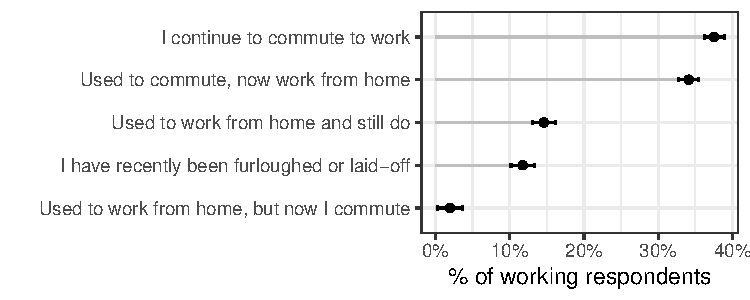
\includegraphics[width = \linewidth]{plots/working_summary.pdf} \\
  \begin{footnotesize}
    %% \begin{singlespace}
    %%   \emph{Notes:} 
    %% \end{singlespace}
    \end{footnotesize}
\end{minipage}
\end{figure} 

GCS also infers respondent gender.
We analyzed responses by gender but did not find any notable differences.
See Appendix~\ref{sec:gender} for this analysis. 

\subsection{Geographic variation} 
COVID-19 has affected various parts of the US differently, with the main epicenter in New York City.
In Figure~\ref{fig:region}, we plot the fraction of respondents choosing each answer by region.
GCS captures a respondent's city and state, which are then mapped to the regions ``Northeast'', ``Midwest'', ``West'', and ``South.'' 

In the first facet from the left, we can see that the South has the highest fraction still commuting to work and the Northeast has the lowest. 
In the second facet from the right, we can see that the Northeast has the highest fraction of respondents switching to working from home, and the South has the fewest.
The Northeast started from the lowest fraction working from home, though these fractions are imprecisely estimated and are all fairly similar to each other. 
The Northeast fraction now working from home is over 40\%. 

\begin{figure}
  \caption{Responses by US region} \label{fig:region}
\centering
\begin{minipage}{1.0 \linewidth}
  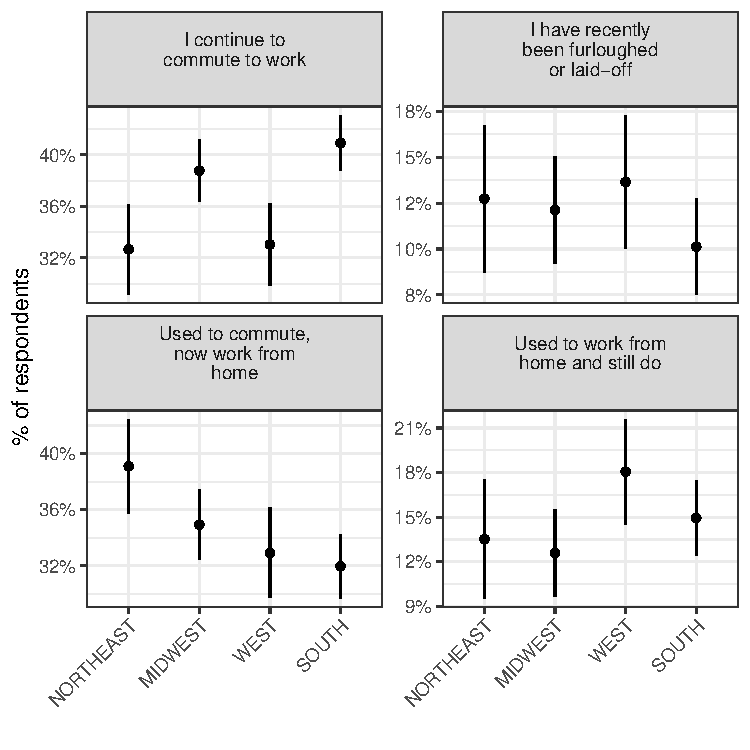
\includegraphics[width = \linewidth]{plots/region.pdf} \\
  \begin{footnotesize}
%    \begin{singlespace}
%      \emph{Notes:} Standard errors are reported. 
%    \end{singlespace}
    \end{footnotesize}
\end{minipage}
\end{figure} 

For a finer-grained look, we plot responses by state.
In Figure~\ref{fig:geo_wfh} we plot the fraction of respondents that switched to working remotely. 
As we saw in Figure~\ref{fig:region}, the highest fractions now working from home are in the Northeast.
The South and parts of the Midwest show substantially less remote work. 
.\footnote{
  We provide larger maps for each fraction in Appendix~\ref{sec:maps}. 
}
It is important to keep in mind that some of these point estimates are fairly imprecise.


\subsection{By gender} \label{sec:gender}

In Figure~\ref{fig:gender} we report responses by inferred gender.
Fractions are computed separately for males and females, and then a slope graph is used to show differences. Within all questions at a 95\% confidence interval, the differences between gender are not statistically significant. Within our sample, however, it appears that men were modestly more likely to continue to commute to work, and likewise women more were more likely to report switching from commuter to work from home status. Men were also slightly more likely to have been recently furloughed or laid-off. Consistently working from home workers show little different in gender composition.

\begin{figure}
  \caption{Responses by gender} \label{fig:gender}
\centering
\begin{minipage}{1.0 \linewidth}
  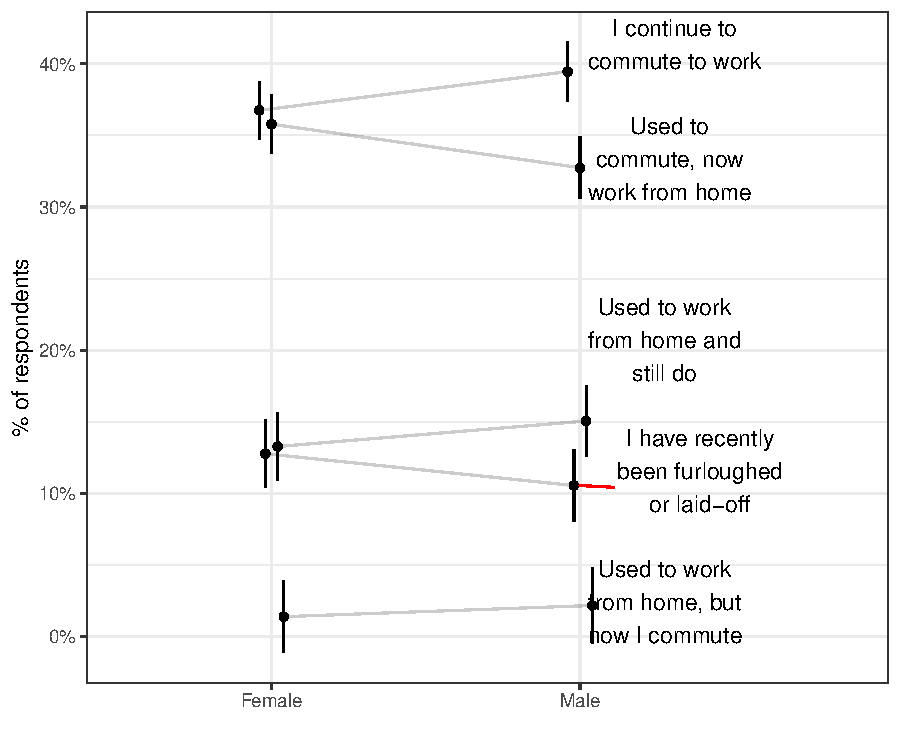
\includegraphics[width = \linewidth]{plots/gender.pdf} \\
  \begin{footnotesize}
    \begin{singlespace}
 %     \emph{Notes:} Standard errors are reported. 
    \end{singlespace}
    \end{footnotesize}
\end{minipage}
\end{figure} 


In Figure~\ref{fig:by_age} we report responses by inferred age.
A similar proportion of workers continue to commute to work across all age groups, as is also the case for the recently furloughed or laid-off worker contingent.
On the other hand, the proportion of respondents that has recently converted from commuting to work to remote work steadily declines from the 25-34 age group to the 65 and older category. The differences between the 25-34 age group and the 65 and older group are statistically significant, and, as Figure~\ref{fig:by_age} shows, younger workers (above age 25) are more likely to have been converted to work from home from commuting. 

Survey respondents in older age groups also reported \emph{remaining} working remotely with greater propensities.
These results are directionally consistent with the 2019 Census~\cite{ACSTableB08101}, though our estimates are larger.
The differences may arise from a difference in the question asked.
The Census asks about how workers get to work. The 2019 Upwork ``Freelancing in America'' study found younger workers were modestly \emph{more} likely to work mostly or entirely from home~\cite{upwork2019}.
It is possible that our survey is somewhere in between, grouping people who do some work at home with those who are fully committed remote labor.
We will investigate further in future work.

\begin{figure}
  \caption{Responses by inferred age} \label{fig:by_age}
\centering
\begin{minipage}{1.0 \linewidth}
  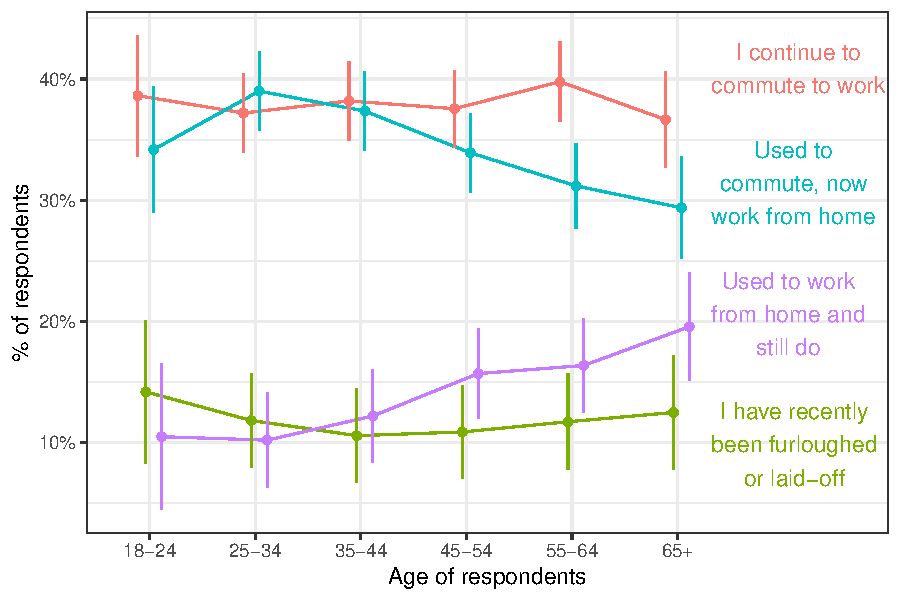
\includegraphics[width = \linewidth]{plots/by_age.pdf} \\
  \begin{footnotesize}
    \begin{singlespace}
 %     \emph{Notes:} Standard errors are reported. 
    \end{singlespace}
    \end{footnotesize}
\end{minipage}
\end{figure} 


%The fraction of workers that are still continuing to commute to work is highest in the Dakotas, Wyoming, and Montana.
%There is still a substantial fraction in the South continuing to commute. 
%The Northeast, with the exception of Vermont, shows large reductions in people still commuting to work. 

\begin{figure}
  \caption{Fraction now working remotely, by US State} \label{fig:geo_wfh}
\centering
\begin{minipage}{1.0 \linewidth}
  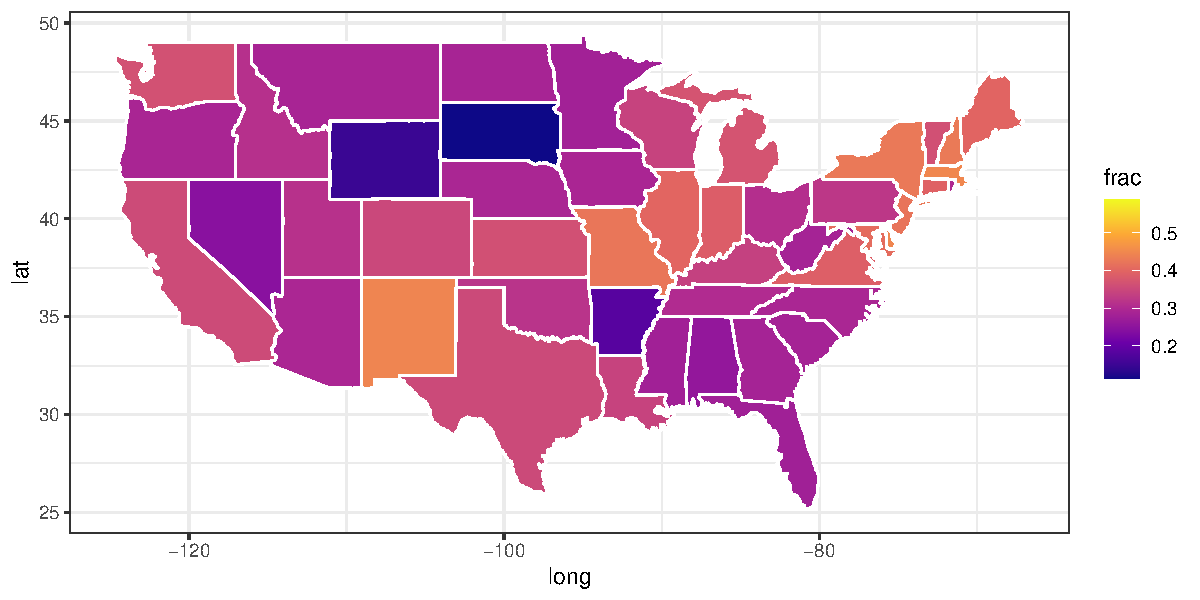
\includegraphics[width = \linewidth]{plots/geo_wfh.pdf} \\
  \begin{footnotesize}
    \end{footnotesize}
\end{minipage}
\end{figure} 

The fractions laid-off or furloughed by US State are shown in Figure~\ref{fig:geo_laidoff}.

\begin{figure}
  \caption{Fraction Laid-off/furloughed, by US State} \label{fig:geo_laidoff}
\centering
\begin{minipage}{1.0 \linewidth}
  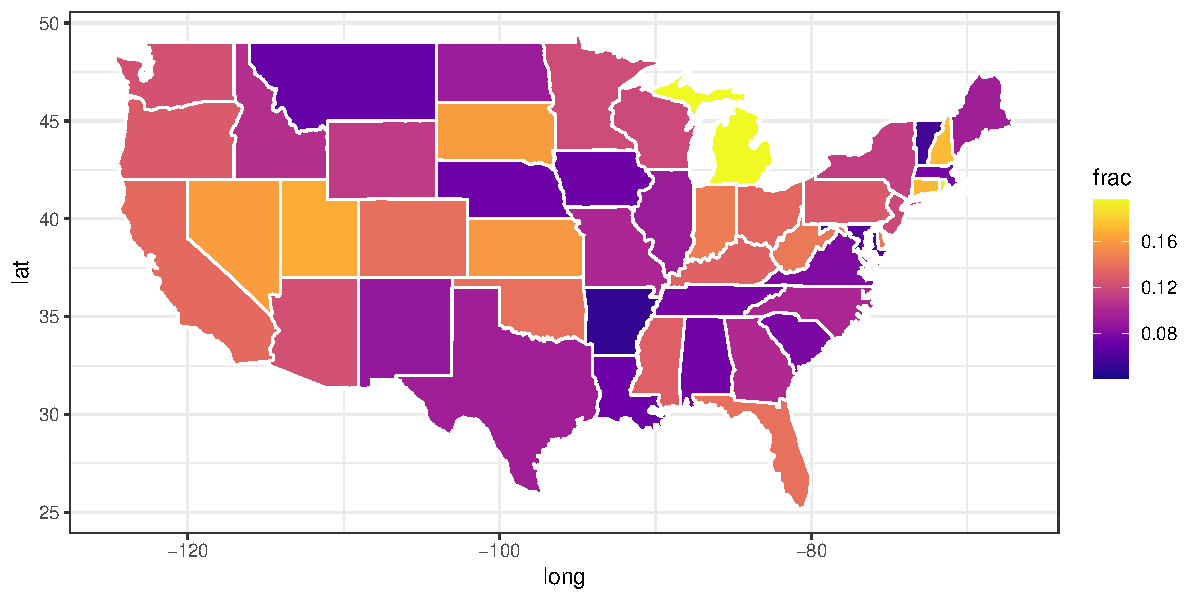
\includegraphics[width = \linewidth]{plots/geo_laidoff.pdf} \\
  \begin{footnotesize}
    \end{footnotesize}
\end{minipage}
\end{figure} 


In Figure~\ref{fig:commute_vs_wfh} we plot the fraction of respondents working from home versus the fraction still commuting by US state.
There is a clear negative relationship, suggesting a fraction of current commuters will likely---or could---transition to work-from-home status.
Each 10 percentage point increase in the fraction still commuting is associated with about a 6 percentage point decline in the fraction of workers now working from home. 

\begin{figure}
  \caption{Still commuting versus work from home fractions by US State} \label{fig:commute_vs_wfh}
\centering
\begin{minipage}{0.8 \linewidth}
  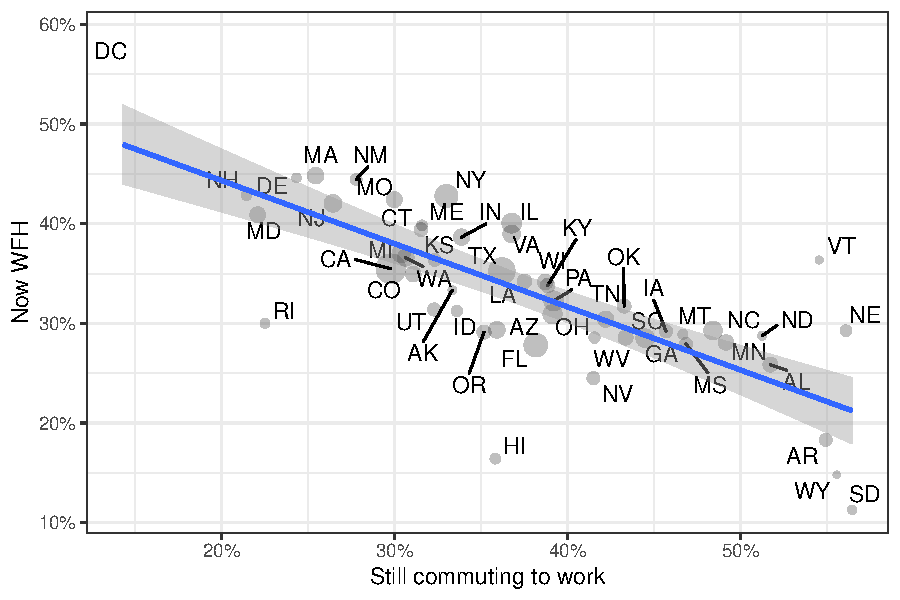
\includegraphics[width = \linewidth]{plots/commute_vs_wfh.pdf} \\
  \begin{footnotesize}
    %% \begin{singlespace}
    %%   \emph{Notes:} 
    %% \end{singlespace}
    \end{footnotesize}
\end{minipage}
\end{figure} 

Table~\ref{tab:remotework} documents heterogeneity in the incidence of COVID (measured as the log of cases per 100,000 individuals\footnote{Data accessed on April 5, 2020 from The New York Times website: https://www.nytimes.com/interactive/2020/us/coronavirus-us-cases.html\#states}) as being strongly positively predictive of switching to remote work and negatively predictive of continuing to commute.

\begin{table}[!htbp] \centering 
  \caption{Predicting remote work by state incidence of COVID-19} 
  \label{tab:remotework} 
\small 
\begin{tabular}{@{\extracolsep{5pt}}lccc} 
\\[-1.8ex]\hline 
\hline \\[-1.8ex] 
 & \multicolumn{3}{c}{\textit{Dependent variable:}} \\ 
 \cline{2-4} 
 & (1) & (2) & (3) \\
 \\[-1.8ex] & Work from home & Continue to commute & Furloughed or laid-off \\ 
 \\[-1.8ex] & (1) & (2) & (3) \\ 
\hline \\[-1.8ex] 
Log cases per 100k pop & 0.0501$^{***}$ & -0.0545$^{***}$ & -0.000305 \\
 & (0.0116) & (0.0147) & (0.00700) \\
Constant & 0.136$^{***}$ & 0.590$^{***}$ & 0.122$^{***}$\\
 & (0.0472) & (0.0590) & (0.0275) \\
 &  &  &  \\
Observations & 51 & 51 & 51 \\
 R$^{2}$ & 0.230 & 0.188 & 0.000 \\ \hline
\hline 
\hline \\[-1.8ex] 
\end{tabular}
\\
\begin{minipage}{1.0 \textwidth}
{\footnotesize \emph{Notes}: 
\starlanguage}
\end{minipage}
\end{table}


A natural question is how these various measures are affecting UI claims by state. 
In Table~\ref{tab:ui}, we combine our data with that on UI claims from \cite{goldsmith2020}.
We regress the log of two weeks of UI claims in a state on the state's population and the log state-specific fraction for each of the response possibilities.  
Unsurprisingly, across all specifications, the state population explains a great deal of the variation in UI claims.
We are interested in asking whether our survey measures account for some of the residual variation.

\begin{table}[!htbp] \centering                    \caption{Predicting UI claims by state}                    \label{tab:ui}                  \small                  \begin{tabular}{@{\extracolsep{5pt}}lcccc}                  \\[-1.8ex]\hline                  \hline \\[-1.8ex]                   & \multicolumn{4}{c}{\textit{Dependent variable:}} \\                  \cline{2-5}                  \\[-1.8ex] & \multicolumn{4}{c}{Log state six week UI claims} \\                  \\[-1.8ex] & (1) & (2) & (3) & (4)\\                  \hline \\[-1.8ex]               
 \\
[1em]
Log of state        &       1.012\sym{***}&       1.019\sym{***}&       1.013\sym{***}&       1.125\sym{***}\\
population          &     (0.035)         &     (0.042)         &     (0.033)         &     (0.061)         \\
[1em]
Log of LFPR         &      -0.554         &      -0.492         &       0.249         &       0.154         \\
                    &     (0.408)         &     (0.499)         &     (0.470)         &     (0.526)         \\
[1em]
Still commuting     &      -1.666\sym{***}&                     &                     &                     \\
frac. (log)         &     (0.473)         &                     &                     &                     \\
[1em]
Now WFH frac. (log) &                     &       0.671         &                     &                     \\
                    &                     &     (0.708)         &                     &                     \\
[1em]
Laid-off frac. (log)&                     &                     &       2.940\sym{***}&                     \\
                    &                     &                     &     (0.673)         &                     \\
[1em]
Still WFH (log)     &                     &                     &                     &      -0.004\sym{**} \\
                    &                     &                     &                     &     (0.002)         \\
[1em]
Constant            &      -2.304\sym{***}&      -3.221\sym{***}&      -2.765\sym{***}&      -4.052\sym{***}\\
                    &     (0.519)         &     (0.788)         &     (0.553)         &     (0.793)         \\
[1em]
Observations        &          51         &          51         &          51         &          51         \\
\(R^{2}\)           &        0.95         &        0.93         &        0.94         &        0.93         \\
\hline                  \hline \\[-1.8ex]                  \end{tabular}                 \\                 \begin{minipage}{1.0 \textwidth}                 {\footnotesize \emph{Notes}:                 \starlanguage}                 \end{minipage}                 \end{table}


In Column~(1), we append the state-specific fraction reporting that they were still commuting to work.
The higher the fraction reporting still commuting, the lower the UI claims for that state.
In Column~(2), the greater the fraction that reports working from home, the \emph{higher} the UI claims.
What seems likely is that workers who would otherwise be continuing to commute to work are splitting into (a) work-from-home or (b) filing for UI.
As states impose further restrictions on mobility, we should be able to get a sense of the resulting increases in UI filings based on how many workers can be successfully transitioned to remote work. 
Surprisingly, Column~(3), which includes a direct measure of reported lay-offs has the ``right'' sign, but is small in magnitude.
%How much of this is due to Michigan - a potential outlier? Or other state-specific effects?
We will investigate this further.

\section{Conclusion}
We document some early facts about how the US labor force is responding to COVID-19 pandemic.
We will continue to track changes to the nature of remote work, asking how pandemic-induced changes transform workplaces in the short and long-term.

\subsection{Suggested immediate future work} 

\begin{itemize}
\item How are state-specific occupational distributions affecting the share of workers able to perform remote work? And to what effect on the UI system? 
\item Are COVID-19 deaths/hospitalizations affecting the adoption of remote work down the distribution of occupations based upon their ``remote-ability''? What are the implications for productivity?
\item Can we predict how UI claims evolve in states based on how much of the workforce they can successfully shift to remote work? 
\item What percentage of tasks can be done remotely and how does it vary across professions and industries? Can we also observe (and explain) heterogeneity across states? These task specific questions will be the focus of our next round of surveys. 
\end{itemize}

The code and data for this project are here:

\href{https://github.com/johnjosephhorton/remote\_work/}{https://github.com/johnjosephhorton/remote\_work/}.

\newpage \clearpage
\bibliographystyle{aer}
\bibliography{remote_work.bib}







%% \subsection{Better looking maps} \label{sec:maps}

%% \begin{figure}
%%   \caption{Responses by US State} \label{fig:geo}
%% \centering
%% \begin{minipage}{1.0 \linewidth}
%%   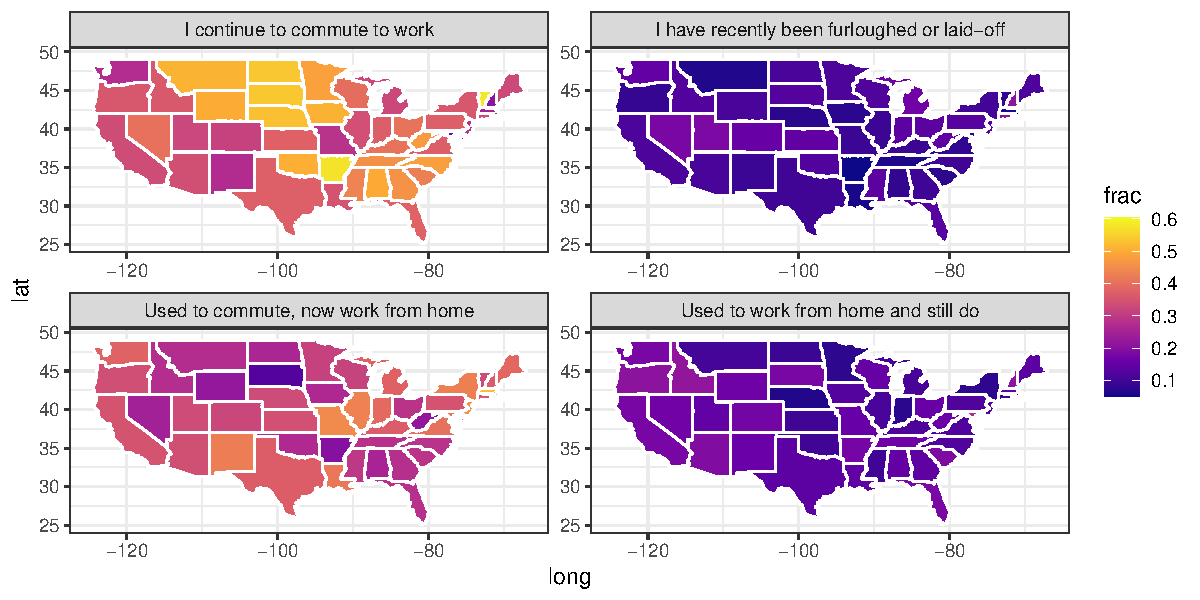
\includegraphics[width = \linewidth]{plots/geo.pdf} \\
%%   \begin{footnotesize}
%%     %% \begin{singlespace}
%%     %%   \emph{Notes:} 
%%     %% \end{singlespace}
%%     \end{footnotesize}
%% \end{minipage}
%% \end{figure} 

%% \begin{figure}
%%   \caption{Laid-off/furloughed by US State} \label{fig:gender}
%% \centering
%% \begin{minipage}{1.0 \linewidth}
%%   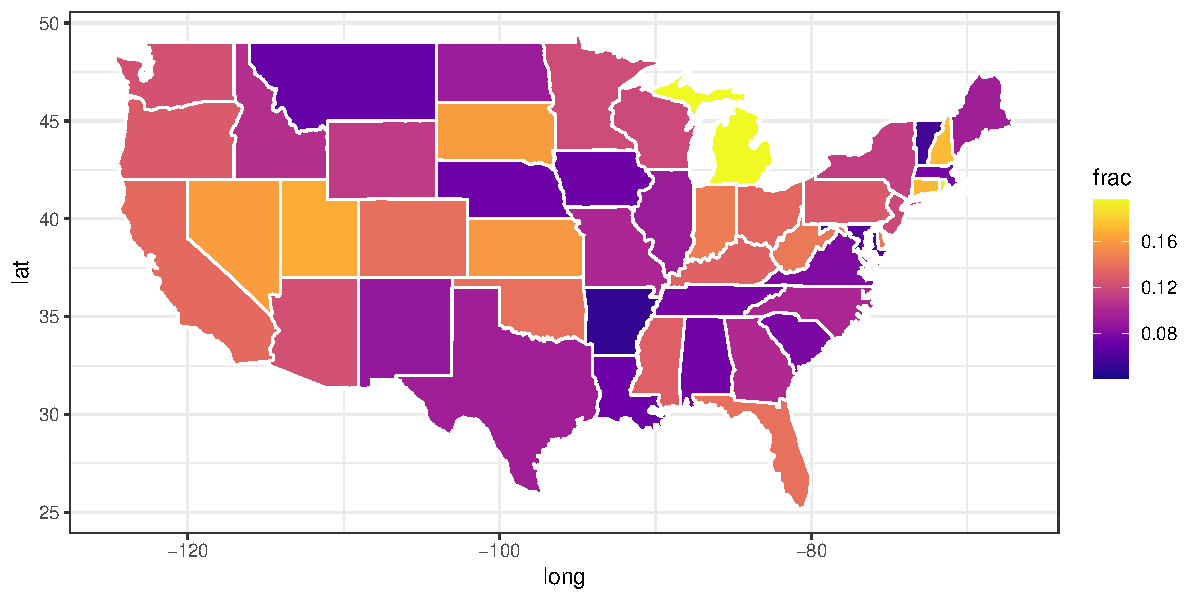
\includegraphics[width = \linewidth]{plots/geo_laidoff.pdf} \\
%%   \begin{footnotesize}
%%     \end{footnotesize}
%% \end{minipage}
%% \end{figure} 


%% \begin{figure}
%%   \caption{Now work-from-home by US State} \label{fig:wfh}
%% \centering
%% \begin{minipage}{1.0 \linewidth}
%%   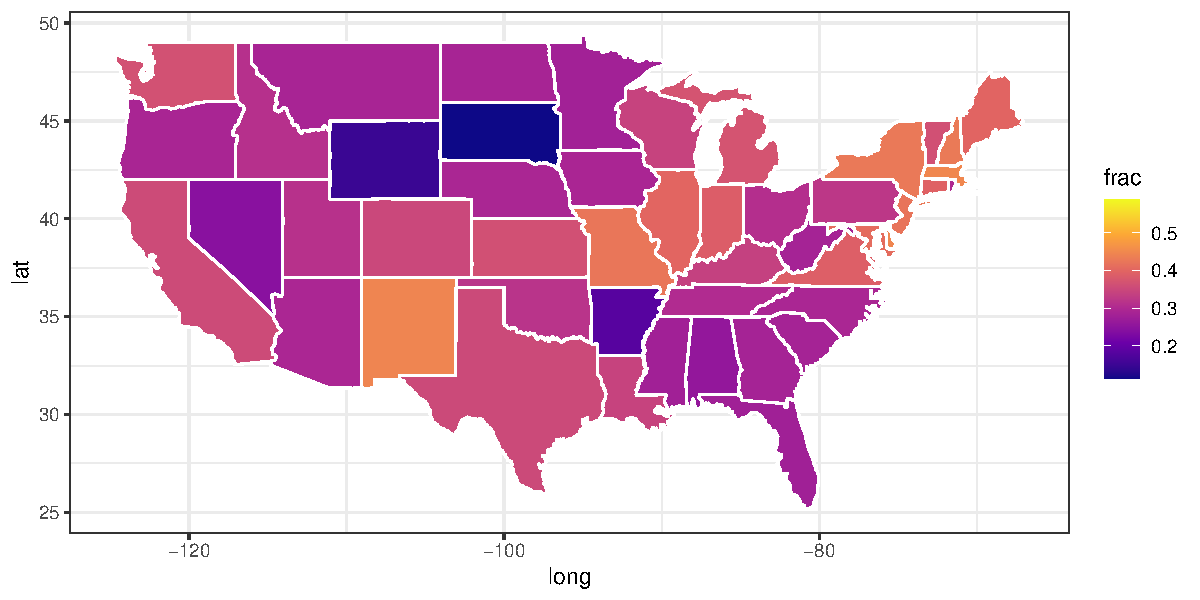
\includegraphics[width = \linewidth]{plots/geo_wfh.pdf} \\
%%   \begin{footnotesize}
%%     \end{footnotesize}
%% \end{minipage}
%% \end{figure} 

%% \begin{figure}
%%   \caption{Still commuting to work by US State} \label{fig:geo_still_commuting}
%% \centering
%% \begin{minipage}{1.0 \linewidth}
%%   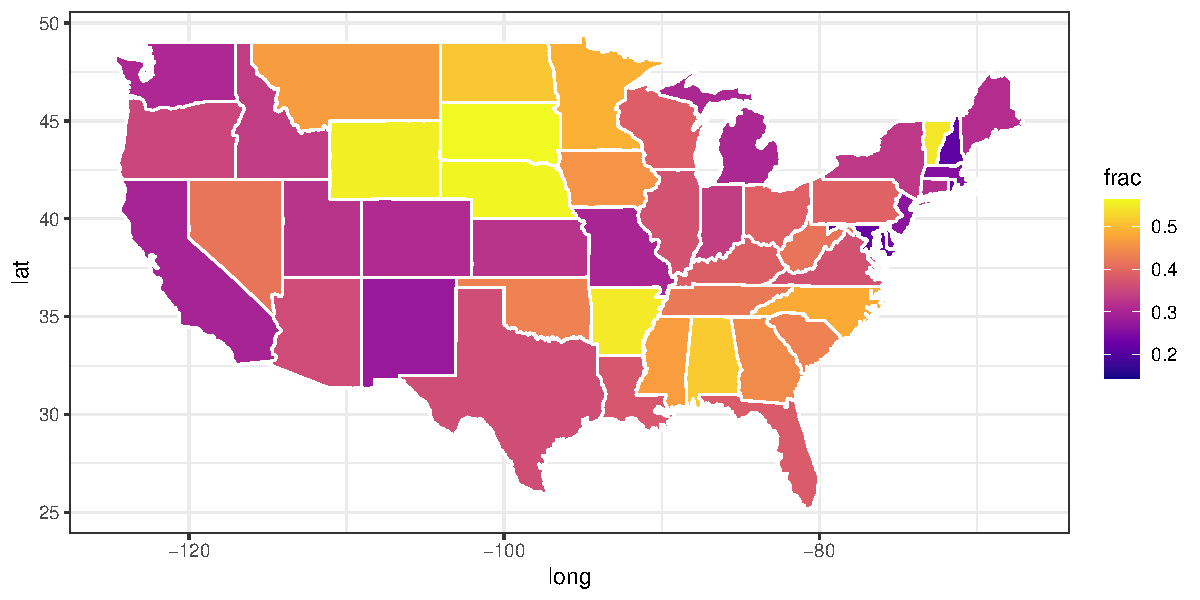
\includegraphics[width = \linewidth]{plots/geo_still_commuting.pdf} \\
%%   \begin{footnotesize}
%%     \end{footnotesize}
%% \end{minipage}
%% \end{figure} 


\end{document} 
